\section{Funciones anónimas}
\begin{frame}
  \frametitle{Funciones anónimas}
  Las \textbf{funciones anónimas} son funciones que no tienen identificador. Usos:
  \begin{itemize}
  \item Como argumentos de funciones de orden superior.
  \item Para construir el resultado de funciones de orden superior.
  \end{itemize}
  Su sintaxis es la siguiente:
  \inputminted[bgcolor=bg]{haskell}{code/anon.hs}
  Donde:
  \begin{itemize}
  \item \texttt{\textbackslash} indica el comienzo de la función.
  \item Entre \texttt{\textbackslash} y \texttt{->} se encuentran sus argumentos.
  \item Detrás de \texttt{->} se encuentra el cuerpo de la función.
  \end{itemize}
\end{frame}

\section{Recursos adicionales}
\begin{frame}
  \frametitle{Recursos adicionales}
  \begin{columns}
    \begin{column}{0.5\textwidth}
      \textbf{\textit{Learn You a Haskell for Great Good!}}\\
      \url{http://learnyouahaskell.com/chapters}
    \end{column}
    \begin{column}{0.5\textwidth}  %%<--- here
      \begin{center}
        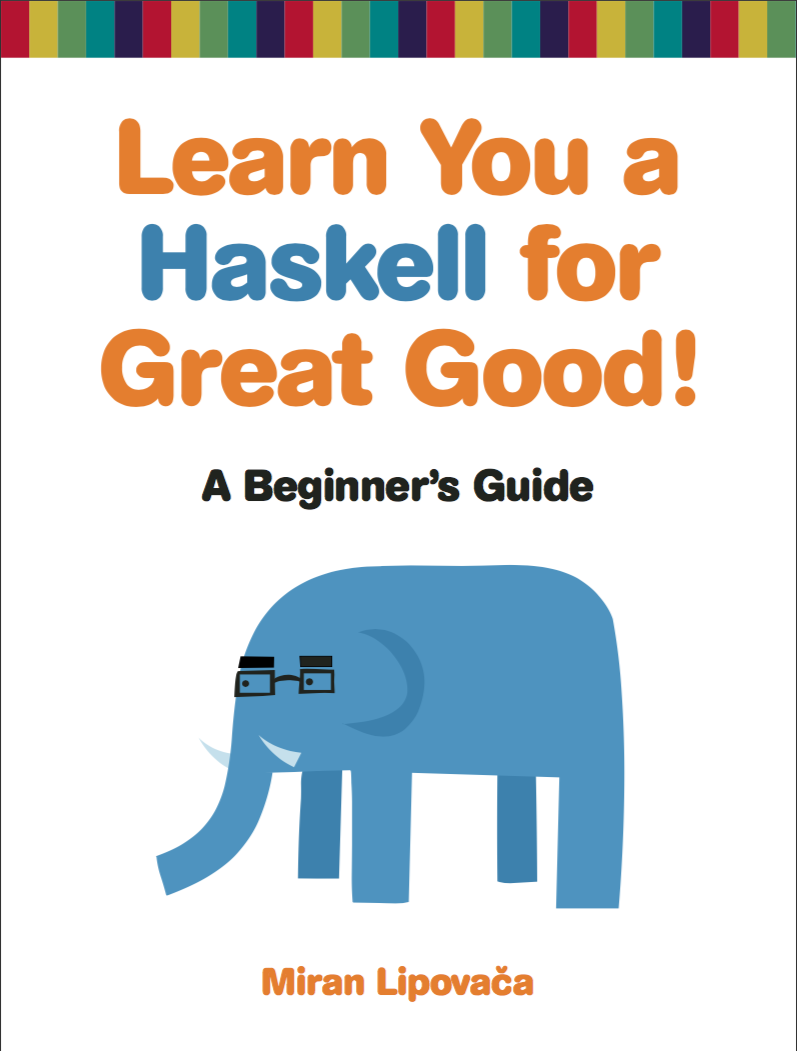
\includegraphics[width=0.5\textwidth]{img/LYH.png}
      \end{center}
    \end{column}
  \end{columns}
\end{frame}
